%%%%%%%%%%%%%%%%%%%%%%%%%%%%%%%%%%%%%%%%%%%%%%%%%%%%%%%%%%%%%%%%%%%%%%
% How to use writeLaTeX: 
%
% You edit the source code here on the left, and the preview on the
% right shows you the result within a few seconds.
%
% Bookmark this page and share the URL with your co-authors. They can
% edit at the same time!
%
% You can upload figures, bibliographies, custom classes and
% styles using the files menu.
%
%%%%%%%%%%%%%%%%%%%%%%%%%%%%%%%%%%%%%%%%%%%%%%%%%%%%%%%%%%%%%%%%%%%%%%

\documentclass[12pt]{article}

\usepackage{sbc-template}

\usepackage{graphicx,url}

%\usepackage[brazil]{babel}   
\usepackage[utf8]{inputenc}
\usepackage{xspace}
\newcommand{\ie}{\emph{i.e.,}\xspace}
\newcommand{\eg}{\emph{e.g.,}\xspace}
\newcommand{\etal}{\emph{et al.}\xspace}
\newcommand{\etc}{\emph{etc.}\xspace}

\sloppy

\title{Instructions for Authors of SBC Conferences\\ Papers and Abstracts}

\author{Diego Dimer Rodrigues\inst{1}, Mariana R Mendoza\inst{1}}


\address{Instituto de Informática -- Universidade Federal do Rio Grande do Sul
  (UFRGS)\\
  Caixa Postal 15.064 -- 91.501-970 -- Porto Alegre -- RS -- Brazil
  \email{\{ddrodrigues,mrmendoza\}@inf.ufrgs.br}
}

\begin{document} 

\maketitle

\begin{abstract}
  This meta-paper describes the style to be used in articles and short papers
  for SBC conferences. For papers in English, you should add just an abstract
  while for the papers in Portuguese, we also ask for an abstract in
  Portuguese (``resumo''). In both cases, abstracts should not have more than
  10 lines and must be in the first page of the paper.
\end{abstract}
     
\section{Introduction}
Machine learning (ML) is increasingly used in various domains, including Health, where it assists in diagnosis, prognosis, and treatment \cite{Chen2021}. 
However, ML algorithms can potentially introduce biases, leading to unfair and potentially harmful outcomes \cite{obermeyer2019dissecting,juhn2022assessing}. 

This work aims to measure the risk of bias in Health datasets using pre-training bias metrics and assesses their impact on the performance of supervised ML algorithms, correlating the bias metrics to the overall models' performance. 
We analyze four pre-training bias metrics \cite{Hardt2021}: Class Imbalance (CI), Kullback-Leibler (KL) Divergence, Kolmogorov-Smirnov (KS), and Conditional Demographic Disparity in Labels (CDDL).

\subsection{Class Imbalance (CI)}
CI measures the representation of different classes within a dataset. It ranges from -1 to 1, with values near zero indicating balanced representation. Positive values indicate overrepresentation of the advantaged group, while negative values indicate overrepresentation of the disadvantaged group.

\subsection{Kullback-Leibler (KL) Divergence}
KL Divergence measures the divergence between the label distributions of two facets. It ranges from 0 to $+\infty$, with values near zero indicating similar distributions and higher values indicating greater divergence.

\subsection{Kolmogorov-Smirnov (KS)}
KS measures the maximum divergence between labels in the distribution for different facets. It ranges from 0 to 1, with values near zero indicating evenly distributed labels and values near one indicating unbalanced labels.

\subsection{Conditional Demographic Disparity in Labels (CDDL)}
CDDL measures the proportion of negative outcomes in a specific facet of a dataset. It ranges from -1 to 1, with positive values indicating demographic disparity favoring the advantaged group and negative values indicating disparity favoring the disadvantaged group.


% \begin{figure}[ht]
% \centering
% \includegraphics[width=.5\textwidth]{fig1.jpg}
% \caption{A typical figure}
% \label{fig:exampleFig1}
% \end{figure}

% \begin{figure}[ht]
% \centering
% \includegraphics[width=.3\textwidth]{fig2.jpg}
% \caption{This figure is an example of a figure caption taking more than one
%   line and justified considering margins mentioned in Section~\ref{sec:figs}.}
% \label{fig:exampleFig2}
% \end{figure}



% \begin{table}[ht]
% \centering
% \caption{Variables to be considered on the evaluation of interaction
%   techniques}
% \label{tab:exTable1}
% 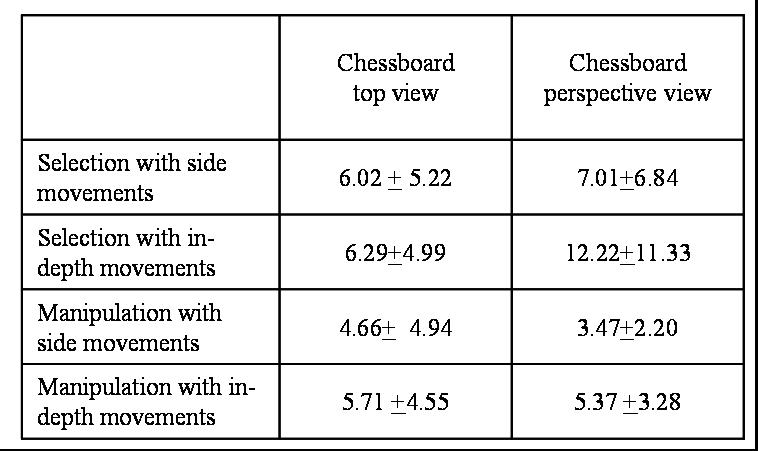
\includegraphics[width=.7\textwidth]{table.jpg}
% \end{table}



\section{References}



\bibliographystyle{sbc}
\bibliography{sbc-template}

\end{document}
